\chapter{Метод сопоставления планов выполнения для автоматического подбора подсказок планировщику}\label{ch:ch3}
\section{Введение}

Современные СУБД предоставляют механизм подсказок оптимизатору, то есть директивы в тексте SQL, направляющие выбор стратегий планирования, от фиксации порядка соединений до предпочтения хеш-соединений перед альтернативами или принудительного использования индекса для заданного отношения. При достаточной квалификации администратор базы данных способен увести оптимизатор от заведомо неудачных решений и подтолкнуть его к более эффективному плану, например, заставить использовать игнорируемый индекс или ограничить порядок соединений, чтобы избежать неэффективных комбинаций. Сложность заключается в том, что подбор корректных подсказок крайне нетривиален и требует глубокого понимания запроса, данных и эвристик оптимизатора, а некорректная подсказка может ухудшить производительность.

Эти трудности стимулировали интерес к автоматизации оптимизации запросов методами машинного обучения. Распространённый подход состоит в том, чтобы рассматривать оптимизатор как «чёрный ящик» и помогать ему подсказками или точечными корректировками выбора плана, добиваясь ускорения без полной замены оптимизатора. Недавние работы показывают, что большие языковые модели (Large Language Model, LLM) способны расширить инструментарий оптимизации запросов, их используют для генерации альтернативных планов и формирования подсказок оптимизатору запросов. Вместе с тем практическое внедрение генеративных LLM-подходов сдерживается стоимостью и временем инференса, что ограничивает применимость в ресурсно чувствительных и требовательных к задержкам сценариях.

В данной главе рассматривается простой метод, использующий эмбеддинги LLM не для самих запросов, а для \emph{планов выполнения}, с целью выбора наборов подсказок оптимизатору. Подход сочетает выразительность эмбеддингов с быстрым «аналогий-ориентированным» механизмом принятия решений и не требует обучения, поскольку вычислительно затратная часть сведена к получению векторного представления плана предобученной моделью.

Для проверки подхода реализован прототип на базе \emph{openGauss} и проведена оценка на стандартном бенчмарке JOB-CEB, включающем 3133 экземпляра запросов из 16 шаблонов на датасете IMDB. В экспериментах метод успешно направлял оптимизатор к более быстрым планам для значительной доли запросов. Результаты показывают, что использование эмбеддингов планов для выбора подсказок способно стабильно превосходить поведение оптимизатора по умолчанию, без сложного обучения и без модификаций базовой системы.

Цель главы состоит в том, чтобы продемонстрировать практическую ценность эмбеддингов планов выполнения и жизнеспособность простой и устойчивой системы вокруг них, ориентированной на применение в реальных нагрузках. Метод намеренно легковесен и не требует обучения, мы используем предобученную модель для получения эмбеддингов планов и применяем поиск ближайших соседей для переноса наборов подсказок. Несмотря на простоту, подход оказывается эффективным, одни лишь эмбеддинги планов сопоставимы по качеству, а в ряде случаев превосходят вручную спроектированные кодировки планов, при существенно меньших инженерных затратах.

Дополнительно проведён эксперимент, направленный на проверку того, что эмбеддинги могут выступать практичной альтернативой ручному кодированию планов выполнения без ухудшения качества. В рамках эксперимента протестированы несколько открытых моделей эмбеддингов, а также несколько вариантов текстового представления плана, подаваемого на вход эмбеддеру. Сравнение выполнено на том же датасете JOB-CEB и включает оценку как ранжирования запросов по времени выполнения, так и точности предсказания времени. Полученные результаты показывают, что при корректном выборе модели и формы представления планы, закодированные только через эмбеддинги, обеспечивают сопоставимое качество по сравнению с ручными признаковыми описаниями, подтверждая возможность снижения объёма ручной инженерии без потери эффективности.

Принципиально важно, что рассматриваемый подход избегает сложности и вычислительных накладных расходов генеративных методов на основе LLM. Использование только эмбеддингов планов существенно дешевле и быстрее, чем генерация планов или правил переписывания, что делает решение более практичным для внедрения. Компонент поиска ближайших соседей также отличается устойчивостью и интерпретируемостью и представляет собой «plug-and-play» механизм, который может быть адаптирован к новым нагрузкам, схемам и распределениям данных.

\section{Постановка задачи}\label{sec:ch3/sec2}

\subsection{Постановка задачи сопоставления планов}

Мы формализуем задачу автоматического выбора хинтов для оптимизации запросов следующим образом. Пусть $Q$ — SQL-запрос, поданный в систему. Оптимизатор запросов может построить для $Q$ план выполнения $P$, которому соответствует некоторая стоимость $C(Q, P)$. В конфигурации по умолчанию (без хинтов) оптимизатор выбирает план $P_{\text{default}}$ на основе встроенных эвристик и стоимостных оценок, что даёт время выполнения $T(Q,P_{\text{default}})$ Наша цель — найти для запроса $Q$ набор хинтов $H$ такой, что, руководствуясь $H$ (и, следовательно, выбирая, возможно, иной план $P_H$), оптимизатор минимизирует время выполнения. Формально, требуется:

\begin{equation}
    \label{eq:equation31}
    H^*(Q) = \arg\min_{H \in \mathcal{H}(Q)} \; T\left(Q,\, P_H\right)
\end{equation}

где $\mathcal{H}(Q)$ обозначает множество всех допустимых конфигураций хинтов для запроса $Q$. Иными словами, $H^*(Q)$ — оптимальный набор хинтов, обеспечивающий наименьшую время исполнения для $Q$. Это эквивалентно «направлению» оптимизатора: выбору хинта или набора хинтов, который приводит к самому быстрому плану для данного запроса. На практике множество $\mathcal{H}(Q)$ может быть очень велико. Полный перебор всех комбинаций хинтов быстро становится непрактичным, поэтому мы ускоряем поиск двумя методами.

\paragraph{Порог тайм-аута (fastest-so-far).}
После каждого выполнения плана мы обновляем переменную
\(
  T_{\min} \leftarrow \min\bigl(T_{\min},\,T(Q,P)\bigr)
\)
(изначально \(T_{\min}=T(Q,P_{\text{default}})\)).
Если любой последующий план с хинтами превышает \emph{текущее} \(T_{\min}\),
мы прерываем его выполнение и помечаем соответствующий набор хинтов как
\emph{субоптимальный}. Это позволяет рано отсекать дорогие планы.
\paragraph{Кэширование планов.}
Каждый уникальный физический план кэшируется вместе с измеренным временем исполнения. Когда оптимизатор порождает план, уже присутствующий в кэше, мы переиспользуем сохранённое значение времени исполнения вместо повторного запуска. Это особенно эффективно, когда многие хинты мало влияют или вовсе не влияют на выбранный план.

\medskip
\noindent
Рассматриваются следующие семь бинарных хинтов:

\begin{itemize}
  \item \texttt{enable\_nestloop}
  \item \texttt{enable\_hashjoin}
  \item \texttt{enable\_mergejoin}
  \item \texttt{enable\_seqscan}
  \item \texttt{enable\_indexscan}
  \item \texttt{enable\_indexonlyscan}
  \item \texttt{enable\_bitmapscan}
\end{itemize}
\paragraph{Разрешение коллизий между эквивалентными наборами хинтов.}
Иногда один и тот же физический план \(P\) может быть получен разными конфигурациями
хинтов. Например,
\[
  H_{1} = (0,1,1,1,0,1,1), \quad
  H_{2} = (0,1,1,1,0,1,0),
\]
порождают идентичный план, хотя отличаются лишь последним флагом (\texttt{enable\_bitmapscan}). Здесь \(i\)-й бит соответствует \(i\)-й булевой оператору из списка выше; значение \(1\) отключает соответствующий оператор, а \(0\) оставляет его в состоянии по умолчанию (включённым). Чтобы выбрать уникальный «канонический» набор хинтов, мы предпочитаем конфигурацию, которая отключает \emph{наименьшее} число операторов:
\[
    \widehat{H}(P) \;=\; \arg\min_{H : P_H = P} \sum_{i=1}^{7} h_i.
\]
В приведённом примере предпочтителен \(H_{2}\), поскольку он отключает на одну «ручку» меньше, чем \(H_{1}\). Это правило основано на двух соображениях. \emph{(i)} Если план может быть получен при любом состоянии «ручки», её влияние на эффективность плана невелико; оставляя её включённой, мы избегаем лишних ограничений. \emph{(ii)} Отключение дополнительных операторов сжимает пространство поиска оптимизатора и может ухудшить производительность на запросах или распределениях данных, отличных от обучающей нагрузки. Выбор наиболее «разрешающего» набора хинтов сохраняет как можно больше встроенной экспертизы оптимизатора, одновременно направляя его к желаемому плану (например, к нужному порядку соединений или типу соединения).

Алгоритм~\ref{alg:hint-search} за один проход просматривает всё пространство из $128$ бинарных наборов хинтов, одновременно постепенно ужесточая порог по времени выполнения. Сначала запрос выполняется при включённых всех операторах, чтобы задать начальный таймаут $T_{\min}$ и инициализировать кэш соответствий «план–время выполнения» $\mathcal{C}$. Оставшиеся конфигурации затем распределяются по $w=8$ рабочим потокам. Для каждого набора хинтов оптимизатор строит физический план; если такой план уже наблюдался, его время выполнения извлекается из $\mathcal{C}$ без повторного запуска. В противном случае запрос исполняется с текущим таймаутом $T_{\min}$. Планы, превышающие таймаут, прерываются досрочно, а соответствующие наборы хинтов помечаются как \emph{субоптимальные}. Каждый раз, когда завершается более быстрое исполнение, $T_{\min}$ атомарно обновляется, немедленно ужесточая таймаут для всех ещё выполняющихся потоков. Поскольку медленные планы быстро останавливаются, а повторяющиеся обходятся через кэш, процедура тратит основное время на небольшое число перспективных конфигураций, при этом гарантируя полное покрытие пространства хинтов.

\begin{algorithm}[H]
\caption{Адаптивный поиск хинтов с отсечением по времени выполнения и кэшированием планов}
\label{alg:hint-search}
\begin{algorithmic}[1]                 % ← нумерация строк

% ----- входные и выходные данные -----
\Require Запрос $Q$;
        Полный каталог бинарных хинтов
        $\mathcal{H}=\{H_1,\dots,H_{128}\}$;
        Количество потоков $w \gets 8$
\Ensure порог по времени выполнения $T_{\min}$;
        кэш соответствий «план–время выполнения» $\mathcal{C}$

% ----- инициализация -----------------------------------------------------
\State $T_{\min} \gets \textsc{execute}(Q,\text{default})$
\State $\mathcal{C} \gets \bigl\{\bigl(\textsc{plan}(Q,\text{default}),\,T_{\min}\bigr)\bigr\}$

% ----- параллельный перебор всех наборов подсказок -----------------------
\ForAll{$H \in \mathcal{H}\setminus\{\text{default}\}$ \textbf{in parallel on} $w$ threads}
    \State $P \gets \textsc{plan}(Q,H)$
    \If{$P \in \mathcal{C}$}
        \State $t \gets \mathcal{C}[P]$
    \Else
        \State $t \gets \textsc{execute}(Q,H,\text{timeout}=T_{\min})$
        \If{$t = \textsc{Timeout}$}
            \State пометить $H$ как \emph{субоптимальный}
            \State \textbf{continue}
        \EndIf
        \State $\mathcal{C}[P] \gets t$
    \EndIf
    \State $T_{\min} \gets \min\!\bigl(T_{\min},\,t\bigr)$ \Comment{атомарное обновление}
\EndFor

% ----- результат ---------------------------------------------------------
\State \Return $(T_{\min},\,\mathcal{C})$
\end{algorithmic}
\end{algorithm}

\subsection{Постановка задачи ранжирования запросов по времени выполнения}
\label{subsec:ranking_problem}

В задаче автоматического выбора подсказок требуется для запроса \(Q\) найти такой набор подсказок \(H\), который приводит оптимизатор к плану \(P_H\) с минимальным временем выполнения \(T(Q,P_H)\). Однако прямое сравнение планов по истинному времени требует их исполнения, что дорого и в общем случае неприменимо при большом числе кандидатов. Поэтому на практике необходим \emph{быстрый приближенный сигнал}, позволяющий оценивать и упорядочивать планы по ожидаемой эффективности без выполнения запроса.

Формализуем эту вспомогательную задачу. Пусть задана выборка запросов \(\mathcal{Q}=\{Q_i\}_{i=1}^{N}\) и соответствующие им планы выполнения \(\mathcal{P}=\{P_i\}_{i=1}^{N}\). Для каждого запроса известно измеренное время выполнения \(T_i = T(Q_i,P_i)\). Требуется построить функцию оценки
\begin{equation}
    s(P) \in \mathbb{R},
\end{equation}
которая по плану \(P\) возвращает скалярный показатель, согласованный с истинным временем выполнения. Основное требование задаётся в терминах рангов: если план \(P_a\) исполняется дольше, чем \(P_b\), то его оценка должна быть больше,
\begin{equation}
    \label{eq:rank_monotonicity}
    T(Q,P_a) > T(Q,P_b) \;\Rightarrow\; s(P_a) > s(P_b),
\end{equation}
по крайней мере для «большинства» пар планов в рассматриваемой нагрузке. Таким образом, задача состоит в максимизации качества ранжирования планов по времени выполнения на основе их представления.

В данной главе рассматриваются три варианта построения такого сигнала \(s(P)\):
\begin{itemize}
    \item \textbf{Оценка оптимизатора.} В качестве базовой линии используется стоимостная оценка плана \(C(Q,P)\), извлекаемая из плана после планирования. Этот сигнал доступен без исполнения запроса и отражает внутреннюю модель стоимости оптимизатора.
    \item \textbf{Ручная структурная кодировка плана.} План \(P\) преобразуется в фиксированный набор признаков на уровне узлов дерева плана, после чего обучается модель \(s_{\text{struct}}(P)\), аналогичная подходам семейства BAO.
    \item \textbf{Эмбеддинги плана.} План \(P\) представляется текстом, затем предобученная модель эмбеддингов строит вектор \(e(P)\), а поверх него обучается лёгкая модель \(s_{\text{emb}}(P)\).
\end{itemize}

Хотя обучение моделей \(s_{\text{struct}}\) и \(s_{\text{emb}}\) выполняется как регрессия времени, целевая переменная задаётся в логарифмической шкале для повышения устойчивости к выбросам и широкому диапазону длительностей:
\begin{equation}
    y = \log(1 + T(Q,P)).
\end{equation}
Предсказание интерпретируется как \(\widehat{T}(Q,P)=\exp(\widehat{y})-1\), а ранжирование планов выполняется по значениям \(\widehat{T}\) или \(\widehat{y}\), что эквивалентно монотонному преобразованию.

Качество решения задачи ранжирования оценивается по ранговым метрикам, включая коэффициенты Спирмена и Кендалла между \(\{s(P_i)\}\) и \(\{T_i\}\), а также по точности попарного сравнения, определяемой долей пар \((i,j)\), для которых знак разности оценок совпадает со знаком разности истинных времен. Дополнительно рассматриваются метрики качества верхней части ранжированного списка, поскольку на практике важна корректная идентификация наиболее медленных запросов.

Таким образом, подзадача ранжирования вводится как вспомогательная по отношению к задаче~\eqref{eq:equation31}: она позволяет количественно сравнить различные представления плана и обосновать применение эмбеддингов как источника сигнала, пригодного для переноса подсказок в методе сопоставления планов выполнения.


\section{Алгоритм сопоставления планов}
В этом разделе описываются принцип сопоставления планов (plan mapping), его мотивация и то, как новый план запроса получает хинты из существующего пространства эмбеддингов. Исходя из предположения, что эмбеддинги LLM способны адекватно представлять план запроса, можно построить систему, которая назначает один и тот же набор хинтов похожим планам. Для этого необходимо определить метрику расстояния между планами, при которой планы, находящиеся на заданном расстоянии друг от друга, получают одинаковый набор хинтов.

При планировании запроса с новым хинтом возникает новый, потенциально более быстрый план. Полезно учитывать этот новый план и в самой системе. Следуя этой идее, для потенциально более быстрого плана формируется второй эмбеддинг, который сравнивается с оптимизированным планом, полученным при применении хинта, в хранилище эмбеддингов. Таким образом, назначение хинтов проходит двухэтапную проверку: сначала сравниваются планы по умолчанию и ищется кандидат на хинт, затем оценивается модифицированный план.

Цель состоит в том, чтобы для \emph{нового плана} $P_0$ (полученного для входного запроса $Q$ при включённых всех хинтах) определить, существует ли в пространстве эмбеддингов близкий план, набор хинтов которого с высокой вероятностью улучшит $Q$. Мы работаем в пространстве эмбеддингов планов, формируемых предобученной LLM; ниже слово «план» всегда означает его эмбеддинг.

Из офлайн-поиска, описанного в алгоритме \ref{alg:hint-search}, мы сохраняем тройки \( (\mathbf{d}_i,\,H_i^\star,\,\mathbf{o}_i) \), где $\mathbf{d}_i$ - эмбеддинг $i$-го \emph{плана по умолчанию}, $H_i^\star$ — его оптимальный набор хинтов, а $\mathbf{o}_i$ — эмбеддинг соответствующего \emph{оптимизированного} плана. Если ни один набор хинтов не ускоряет запрос, то $H_i^\star$ — это вектор «всё включено», а $\mathbf{o}_i=\mathbf{d}_i$.

Планы, близкие в пространстве эмбеддингов, как правило, разделяют физическую структуру; следовательно, один и тот же набор хинтов часто остаётся полезным в локальной окрестности. Мы используем эту локальность в два этапа:

\begin{enumerate}
    \item \textbf{Голосование в окрестности.} Среди $N$ ближайших планов по умолчанию выбираем самый популярный набор хинтов, отличный от стандартного. Это опирается на предположение, что структурно похожие планы склонны иметь одни и те же узкие места, поэтому применение хинта, сработавшего у соседей, с высокой вероятностью оптимизирует новый план сходным образом.
    \item \textbf{Проверка согласованности.} Перепланируем запрос с выбранным кандидатом и для обоих — плана по умолчанию и плана с кандидатом — собираем их $K$ ближайших соседей (для всех известны времена выполнения), вычисляем среднее время выполнения в каждой окрестности и сравниваем. Если среднее в окрестности плана с кандидатом меньше, чем у плана по умолчанию, принимаем новый набор хинтов; в противном случае сохраняем исходный.
\end{enumerate}

Этот двухэтапный тест балансирует полноту и надёжность: $N$ ближайших соседей позволяют составить список локально популярных наборов хинтов и выбрать наиболее частотный в качестве кандидата, тогда как проверка с $K$ предотвращает слепое применение хинта, которое могло бы увести оптимизатор в субоптимальную область.

\begin{figure}[ht]
  \centering
  \includegraphics[width=0.8\textwidth]{images/plan_mapping.pdf}
  \caption{Двухэтапный выбор хинтов: голосование среди $N$ ближайших соседей планов по умолчанию для выбора кандидата, затем проверка его полезности по $K$ ближайшим соседям оптимизированного плана.}
  \label{fig:plan_mapping}
\end{figure}

Пусть $\phi(\cdot)$ — это LLM-энкодер, отображающий план запроса в
$d$-мерный вектор. На рис.~\ref{fig:plan_mapping} слева показано
встраивание (эмбеддинг) плана по умолчанию $P_0$ в виде точки $p_0$
вместе с его $N$ ближайшими соседями (полупрозрачный синий). Мы
проводим «голосование» по наборам хинтов этих соседей и выбираем
кандидат $H_{\mathrm{cand}}$. Справа показано встраивание перепланированного
запроса $P_{\mathrm{cand}}$ как $h(p_{0})$ и его $K$ ближайших соседей.
Сравнивая среднее время выполнения в двух $K$-окрестностях — вокруг $p$
(с использованием времён по умолчанию) и вокруг $p_{\mathrm{new}}$ (с
использованием времён для оптимизированных планов) — мы решаем, действительно
ли $H_{\mathrm{cand}}$ улучшает производительность. Эта двухэтапная проверка
максимизирует покрытие хинтов (через голосование в первой $N$-окрестности)
и одновременно защищает от вредных рекомендаций (через согласованность во
второй $K$-окрестности).

\begin{enumerate}
  \item \textbf{Встраивание плана по умолчанию.}
    Вычисляем
    \[
      \mathbf{p}_0 = \phi(P_0),
    \]
    где $P_0$ — план оптимизатора по умолчанию для запроса $Q$.

  \item \textbf{Голосование в окрестности.}
    Находим $N$ ближайших соседей для $\mathbf{p}_0$:
    \[
      \mathcal{N}
      = \bigl\{(\mathbf{d}_i, H_i^\star, t_i)
               \mid i\in\text{top-}N\text{ closest to }\mathbf{p}_0
         \bigr\},
    \]
    где каждый сосед несёт свой набор хинтов $H_i^\star$ и известное время выполнения $t_i$.
    Строим частотную таблицу по всем недефолтным $\{H_i^\star\}$ и выбираем
    самый частотный в качестве $H_{\mathrm{cand}}$; при равенстве частот
    предпочитаем ближайшего по расстоянию $\|\mathbf{p}_0-\mathbf{d}_i\|$.

  \item \textbf{Встраивание плана-кандидата.}
    Применяем $H_{\mathrm{cand}}$ к $Q$, получаем план $P_{\mathrm{cand}}$ и вычисляем
    \[
      \mathbf{p}_{\mathrm{cand}} = \phi(P_{\mathrm{cand}}).
    \]

  \item \textbf{Проверка согласованности по двум $K$-окрестностям.}
    \begin{itemize}
      \item Пусть
        \[
          \mathcal{K}_0
          = \{\mathbf{d}_{0,1}, \dots, \mathbf{d}_{0,K}\}
          \quad\text{и}\quad
          \mathcal{K}_{\mathrm{cand}}
          = \{\mathbf{d}_{\mathrm{cand},1}, \dots, \mathbf{d}_{\mathrm{cand},K}\}
        \]
        — $K$ ближайших соседей для $\mathbf{p}_0$ и $\mathbf{p}_{\mathrm{cand}}$ соответственно.
      \item Извлекаем их известные времена выполнения
        $\{t_{0,1},\dots,t_{0,K}\}$ и $\{t_{\mathrm{cand},1},\dots,t_{\mathrm{cand},K}\}$.
      \item Вычисляем средние времена выполнения
        \[
          \bar t_0
          = \frac1K\sum_{j=1}^K t_{0,j},
          \qquad
          \bar t_{\mathrm{cand}}
          = \frac1K\sum_{j=1}^K t_{\mathrm{cand},j}.
        \]
      \item \emph{Принимаем} $H_{\mathrm{cand}}$, если
        $\bar t_{\mathrm{cand}} < \bar t_0$; иначе \emph{отклоняем} его
        (то есть сохраняем план по умолчанию).
    \end{itemize}
\end{enumerate}


У алгоритма три гиперпараметра:

\begin{itemize}
  \item $N$ — размер окрестности для стадии голосования (\(N=16\) в наших экспериментах);
  \item $K$ — проверка согласованности по двум $K$-окрестностям: малый $K$ отдаёт приоритет ближайшим планам, большой $K$ повышает покрытие и стабильность (\(K=16\) также в наших экспериментах);
  \item метрика расстояния (по умолчанию евклидова).
\end{itemize}


\begin{algorithm}[H]
\caption{Сопоставление планов с проверкой согласованности по двум окрестностям}
\label{alg:plan-mapping2}
\footnotesize
\begin{algorithmic}[1]

\Require новый запрос $Q$;
        эталонное множество
        $\displaystyle
          \mathcal{T}=\{(d_i, H_i^\ast, o_i,
          \,t_i^{\mathrm{def}},\,t_i^{\mathrm{opt}})\}_{i=1}^{M}
        $;
        параметры $N$ (соседи для голосования), $K$ (соседи для согласованности)
\Ensure  набор хинтов $H_{\mathrm{out}}$ \textbf{или} $\varnothing$

\State $P_0 \gets \textsc{plan}\!\bigl(Q,\text{default hints}\bigr)$
\State $\mathbf p_0 \gets \phi(P_0)$
\State $\mathcal{N} \gets$ $N$ ближайших $\{d_i\}$ к $\mathbf p_0$
\vspace{2pt}

\State $H_{\mathrm{cand}} \gets
       \operatorname{mode}\!\bigl\{\,H_i^\ast \mid
       H_i^\ast \neq \mathbf 0,\; (d_i,\dots)\in\mathcal{N}\bigr\}$
\If{$H_{\mathrm{cand}}$ не определён}
    \State \Return $\varnothing$
\EndIf
\vspace{2pt}

\State $P_{\mathrm{cand}} \gets \textsc{plan}(Q,H_{\mathrm{cand}})$
\State $\mathbf p_{\mathrm{cand}} \gets \phi(P_{\mathrm{cand}})$

\State $\mathcal{K}_0 \gets$ $K$ ближайших $\{d_i\}$ к $\mathbf p_0$
\State $\displaystyle
       \bar t_0 \gets \frac1K
       \sum_{(d_i,\dots,t_i^{\mathrm{def}},\dots)\in\mathcal{K}_0}
       t_i^{\mathrm{def}}
       $
\State $\mathcal{K}_{\mathrm{cand}} \gets$
       $K$ ближайших $\{o_i\}$ к $\mathbf p_{\mathrm{cand}}$
\State $\displaystyle
       \bar t_{\mathrm{cand}} \gets \frac1K
       \sum_{(o_i,\dots,t_i^{\mathrm{opt}},\dots)\in\mathcal{K}_{\mathrm{cand}}}
       t_i^{\mathrm{opt}}
       $
\vspace{2pt}

\If{$\bar t_{\mathrm{cand}} < \bar t_0$}
    \State $H_{\mathrm{out}} \gets H_{\mathrm{cand}}$
\Else
    \State $H_{\mathrm{out}} \gets \varnothing$
\EndIf
\State \Return $H_{\mathrm{out}}$
\end{algorithmic}
\end{algorithm}

\begin{figure}[htbp]
  \centering
  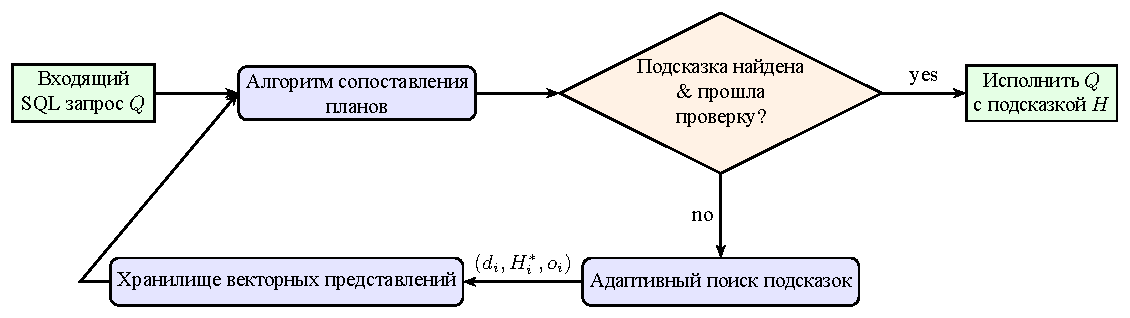
\includegraphics[width=.85\linewidth]{images/overall_design_rus.pdf}
  \caption{Дизайн общей системы}
  \label{fig:overall-system}
\end{figure}

Чтобы эффективно объединить сильные стороны подхода на эмбеддингах, мы интегрируем все предложенные техники в единую конвейерную схему оптимизации запросов. Такая гибридная архитектура призвана (1) обеспечивать быстрое улучшение планов с помощью сопоставления планов, когда в хранилище опыта есть похожие планы из прошлого, (2) при отсутствии подходящих аналогов выполнять тщательный поиск хинтов для «новых» запросов, и (3) со временем повышать общую эффективность за счёт постоянного накопления опыта выполнения запросов. На рисунке \ref{fig:overall-system} показан двухэтапный конвейер оптимизации.

\begin{enumerate}
  \item \textbf{Этап сопоставления планов.}
        Входной SQL-запрос \(Q\) планируется при включённых всех хинтах, затем план встраивается (эмбеддится) и сравнивается с эталонной нагрузкой по алгоритму~\ref{alg:plan-mapping2}.
        Если выбранный кандидат \(H_{\mathrm{cand}}\) проходит проверку согласованности по двум \(K\)-окрестностям, запрос сразу исполняется с \(H_{\mathrm{cand}}\) («быстрый путь»).

  \item \textbf{Резерв: адаптивный поиск хинтов.}
        Когда сопоставление планов не возвращает хинт (или проверка согласованности отклоняет кандидата), \(Q\) передаётся алгоритму~\ref{alg:hint-search}.
        Этот исчерпывающий, но отсечённый по времени выполнения поиск просматривает всё пространство из 128 бинарных наборов хинтов, находит самую быструю конфигурацию и кэширует оптимальную тройку
        \(\langle\text{план по умолчанию}, \text{оптимальный хинт}, \text{оптимизированный план}\rangle\) для последующего использования.

  \item \textbf{Исполнение и непрерывное обучение.}
        Тройки, полученные на резервном шаге, непрерывно расширяют эталонное множество, к которому обращается этап сопоставления планов для каждого нового запроса.
        Со временем эта обратная связь сокращает долю запросов, требующих более медленного полного поиска, устойчиво снижая суммарное время выполнения.
\end{enumerate}

Такая схема обеспечивает низкое медианное время выполнения, поскольку большинство запросов решается легковесным сопоставителем на эмбеддингах, и одновременно гарантирует, что даже «сложные» запросы со временем выигрывают от тщательной процедуры поиска.

\section{BAO-подобные архитектуры для оценки времени выполнения планов}
В данной главе описывается общий подход, использующий ручную кодировку плана выполнения запроса для построения модели предсказания времени его исполнения.

Подход BAO (Bandit Optimizer) относится к семейству методов, которые не заменяют классический оптимизатор, а дополняют его механизмом выбора подсказок. В полной системе BAO предиктивная модель выступает как модуль оценки качества кандидатов и используется внутри более общей схемы выбора подсказок, формулируемой как задача контекстного многорукого бандита. В рамках настоящей главы нас прежде всего интересует сама модель предсказания времени выполнения и способ кодирования планов, так как именно эти элементы задают качество ранжирования и пригодность для переноса знаний между запросами.

Модель получает на вход план выполнения \(P\), задача ставится как задача регрессии. В качестве целевой переменной используется наблюденное время выполнения, измеренное при исполнении плана, то есть \(T(Q,P)\). Предсказание модели \(\widehat{T}(Q,P)\) интерпретируется как оценка качества плана. Далее эта оценка может использоваться как для выбора лучшего кандидата, так и для ранжирования планов и запросов по ожидаемой длительности.

BAO преобразует дерево плана в дерево векторных представлений. Процедура включает два шага.

\begin{enumerate}
    \item \textbf{Приведение к бинарному дереву.}
    Для применения свёртки по дереву исходное дерево плана приводится к строго бинарной форме. Узлы с числом потомков больше двух раскладываются в бинарную структуру, а отсутствующие дети в бинарных узлах дополняются фиктивными потомками типа \texttt{null}. Это унифицирует структуру входа и упрощает последующую обработку.

    \item \textbf{Векторизация узлов.}
    Каждый узел дерева кодируется фиксированным вектором признаков. В базовом варианте BAO используются:
    \begin{itemize}
        \item one-hot кодирование типа физического оператора, например сканирование, сортировка, агрегирование, соединение и т.д.;
        \item числовые оценки оптимизатора, включающие оценку кардинальности и оценку стоимости, то есть два скалярных признака на узел;
    \end{itemize}
    Принципиальная особенность такой кодировки состоит в том, что она опирается на информацию, уже доступную оптимизатору, и избегает явного кодирования имён отношений и атрибутов. Это снижает зависимость модели от конкретной схемы и облегчает переносимость при изменениях структуры данных.
\end{enumerate}

Предиктивная модель BAO реализована как свёрточная нейронная сеть по деревьям (Tree Convolutional Neural Network, TCNN). Обработка дерева выполняется снизу вверх, а параметры свёртки разделяются между всеми узлами, что обеспечивает одинаковое преобразование для одинаковых локальных шаблонов плана.

Пусть на некотором слое нейросети векторное представление узла \(v\) обозначено как \(h_v\), а представления его левого и правого потомков как \(h_{l(v)}\) и \(h_{r(v)}\). Одна tree convolution операция вычисляет новое представление узла по конкатенации трёх векторов:
\begin{equation}
h^{\prime}_v = \sigma\left(W \cdot [h_v,\, h_{l(v)},\, h_{r(v)}] + b\right),
\end{equation}
где \(\sigma(\cdot)\) это нелинейность, а \(W,b\) это обучаемые параметры слоя. В BAO используется несколько последовательных слоёв tree convolution, что позволяет модели учитывать контекст узла на всё большей глубине дерева.

В типичной конфигурации BAO применяется три слоя свертки, затем слой динамической агрегации, который сводит дерево произвольного размера к вектору фиксированной длины. После агрегации используются два полносвязных слоя, отображающие полученное представление в скалярную оценку времени выполнения. Для обучения применяются стандартные практики нейросетевой оптимизации, включая оптимизатор Adam, а также нормализацию между слоями и нелинейности типа ReLU.

Такая архитектура позволяет распознавать структурные шаблоны в планах выполнения, например комбинации операторов сортировки и соединения, а также потенциально неэффективные конструкции, которые проявляются в локальных поддеревьях. Числовые признаки кардинальности и стоимости дают модели сигнал о масштабе операций.

Далее данный подход будет протестирован и сопоставлен с моделью, использующей эмбеддинги планов выполнения, в следующем разделе.

\section{Тестирование предсказательной модели}

В данном разделе оценивается способность различных представлений планов выполнения служить входом для модели, предсказывающей время исполнения запроса и ранжирующей планы по ожидаемой скорости. Эксперименты преследуют три цели.

Во-первых, сравнить два способа текстового представления плана, подаваемого на вход модели эмбеддингов, и определить, какая форма представления устойчивее и информативнее. Во-вторых, сравнить несколько открытых моделей эмбеддингов и выявить, какие из них лучше сохраняют информацию, релевантную для предсказания времени исполнения. В-третьих, сопоставить качество подхода на эмбеддингах с двумя базовыми ориентирами: со стоимостной оценкой оптимизатора и с моделью BAO-подобного класса, использующей ручную кодировку дерева плана.

Оценка проводится на датасете JOB-CEB. Для обеспечения сопоставимости все модели тестируются на одних и тех же разбиениях на обучающую, валидационную и тестовую выборки. Качество рассматривается в двух аспектах: точность предсказания времени исполнения и качество ранжирования планов по ожидаемому времени.

\subsection{Текстовые представления планов}
\label{subsec:plan_text_repr}

В экспериментах используются два текстовых представления планов выполнения.

\textbf{Plain-представление} представляет собой исходный текст \texttt{EXPLAIN}, полученный от СУБД в человекочитаемой форме, без каких-либо преобразований. Данный вариант отражает фактическое отображение плана в СУБД, однако содержит значительную вариативность форматирования и лексики, а также включает множество деталей, не всегда релевантных для задачи ранжирования по времени.

\textbf{Нормализованное представление} строится из \texttt{EXPLAIN (FORMAT JSON)} и предназначено для получения устойчивой к форматированию и токенизации формы плана. Нормализация выполняется как обход дерева плана в порядке preorder с записью одного узла на строку. Каждая строка начинается с индикатора глубины \(L_d\), за которым следует тип физического оператора, а далее фиксированный набор атрибутов узла.

В нормализованном тексте используются только поля, доступные до исполнения запроса, то есть параметры стоимостной модели и сведения о структуре плана. Для числовых параметров \texttt{Total Cost} и \texttt{Plan Rows} применяется логарифмическое бакетирование по основанию 10 с шагом \(0.1\), в результате чего значения представляются токенами вида \(10^{k}\). Дополнительно вычисляется относительная величина \texttt{ct\_frac}, равная отношению \texttt{Total Cost} узла к \texttt{Total Cost} корня, также записываемая в виде логарифмического бакета. Это позволяет отразить масштаб узла относительно всего плана и уменьшить чувствительность к абсолютным значениям стоимости.

Предикатные выражения (например \texttt{Filter}, \texttt{Hash Cond}, \texttt{Index Cond}) нормализуются отдельно: удаляются явные приведения типов, строковые литералы заменяются на маркер \(S\), числовые литералы заменяются на бакеты (отдельно для малых чисел и для больших значений), а выражения вида \texttt{IN (...)} и массивы приводятся к компактной форме \texttt{LIST:len=k}. Такая нормализация уменьшает взрыв словаря токенов, сохраняя при этом информацию о структуре условий и грубом масштабе числовых значений.

Часть потенциально доступных метаданных узлов (например флаги параллелизма или служебные атрибуты) в экспериментах намеренно не включалась в текст, чтобы уменьшить шум и повысить устойчивость представления. В результате нормализованное представление можно рассматривать как каноническую сериализацию дерева плана, ориентированную на стабильность токенов и переносимость между запросами.

\begin{lstlisting}[caption={Пример plain-представления плана (\texttt{EXPLAIN} без нормализации)},label={lst:plan_plain_example}]
Aggregate  (cost=12345.67..12345.68 rows=1 width=8)
  ->  Nested Loop  (cost=12.34..12340.12 rows=1500 width=16)
        Join Filter: (t.id = mi.movie_id)
        ->  Index Scan using title_pkey on title t  (cost=0.42..8.45 rows=1 width=8)
              Index Cond: (id = 1234)
              Filter: (production_year > 2000)
        ->  Bitmap Heap Scan on movie_info mi  (cost=11.90..12200.00 rows=20000 width=8)
              Recheck Cond: (info_type_id = 3)
              Filter: (info = 'USA')
              ->  Bitmap Index Scan on info_type_id_movie_info  (cost=0.00..6.50 rows=20000 width=0)
                    Index Cond: (info_type_id = 3)
\end{lstlisting}

\begin{lstlisting}[caption={Пример нормализованного представления плана (после преобразования)},label={lst:plan_norm_example}]
L0 Aggregate cost=10^4.1..10^4.1 rows=10^0.0 width=8 ct_frac=10^0.0 type=Aggregate
L1 Nested Loop cost=10^1.1..10^4.1 rows=10^3.2 width=16 ct_frac=10^0.0 type=Nested Loop join=Inner cond_joinfilter: (t.id = mi.movie_id)
L2 Index Scan cost=10^-0.4..10^0.9 rows=10^0.0 width=8 ct_frac=10^-3.2 type=Index Scan rel=title idx=title_pkey cond_idx: (id = N:r25=1225) filter: (production_year > N:r25=2000)
L2 Bitmap Heap Scan cost=10^1.1..10^4.1 rows=10^4.3 width=8 ct_frac=10^0.0 type=Bitmap Heap Scan rel=movie_info recheck: (info_type_id = N:small) filter: (info = S)
L3 Bitmap Index Scan cost=0..10^0.8 rows=10^4.3 width=0 ct_frac=10^-3.3 type=Bitmap Index Scan idx=info_type_id_movie_info cond_idx: (info_type_id = N:small)
\end{lstlisting}


\subsection{Модели эмбеддингов}
\label{subsec:embedding_models}

Для оценки универсальности подхода протестированы три открытые модели эмбеддингов.

\begin{itemize}
    \item \textbf{Qwen3-Embedding-0.6B}. Универсальная модель эмбеддингов общего назначения. Рассматривается как представитель современных компактных эмбеддеров, способных устойчиво работать на широком спектре текстов, что важно для переносимости на разные форматы планов.

    \item \textbf{jina-code-embeddings-0.5b}. Модель, ориентированная на код и технические тексты. Используется как представитель специализированных эмбеддеров, которые потенциально лучше захватывают структурные элементы текстов планов, включая названия операторов и типовые шаблоны.

    \item \textbf{BAAI/bge-m3}. Многоязычная модель эмбеддингов, оптимизированная под задачи семантического поиска и сопоставления. Включена как представитель моделей, которые часто демонстрируют высокое качество при поиске ближайших соседей по смыслу, что непосредственно связано с задачами ранжирования и сопоставления планов.
\end{itemize}

Выбор этих моделей позволяет сравнить три характерных сценария: универсальный эмбеддер общего назначения, специализированный эмбеддер для кода и модель, ориентированная на семантическое сопоставление в задачах информационного поиска.

\subsection{Обучение модели ранжирования}
\label{subsec:ranking_training}

На основе эмбеддингов планов обучается компактная нейросетевая модель, предсказывающая время выполнения и задающая ранжирование планов по ожидаемой длительности. Для каждого плана строится эмбеддинг \(x \in \mathbb{R}^d\). Перед обучением выполняются две стандартные процедуры нормализации: L2-нормализация эмбеддингов и стандартизация по статистикам обучающей выборки,
\[
x \leftarrow \frac{x}{\lVert x\rVert_2 + \varepsilon}, \qquad
x \leftarrow \frac{x - \mu}{\sigma},
\]
где \(\mu\) и \(\sigma\) вычисляются по обучающим данным, а \(\varepsilon\) является малой константой для численной устойчивости.

В качестве целевой переменной используется логарифмированное время выполнения:
\[
y = \log(1 + T_{\mathrm{ms}}),
\]
где \(T_{\mathrm{ms}}\) это измеренное время выполнения запроса в миллисекундах. Такой выбор повышает устойчивость обучения, так как распределение времен имеет выраженный длинный правый хвост.

Архитектура модели представляет собой многослойный перцептрон из трёх скрытых слоёв. Каждый скрытый слой состоит из линейного преобразования, нелинейности GELU и метод прореживания для регуляризации. Выходной слой является линейным и возвращает скалярное предсказание \(\hat{y}\). Обучение производится минимизацией среднеквадратичной ошибки,
\[
\mathcal{L} = \lVert \hat{y} - y \rVert_2^2,
\]
с использованием оптимизатора AdamW и L2-регуляризации через затухание весов. Для предотвращения переобучения применяется ранняя остановка по метрике качества на валидационной выборке.

Хотя модель обучается как регрессор времени, она также используется как модель ранжирования: планы упорядочиваются по \(\hat{y}\) или эквивалентно по \(\widehat{T}_{\mathrm{ms}}=\exp(\hat{y})-1\), после чего вычисляются ранговые метрики качества.

Для корректной оценки обобщающей способности модели использовались два режима разбиения датасета на обучающую и тестовую части.

Первый режим представляет собой стандартную \(K\)-кратную кросс-валидацию со случайным разбиением запросов (в работе использовано \(K=5\)). Такой протокол оценивает качество в ситуации, когда распределения обучающих и тестовых примеров близки, то есть тестовая выборка содержит запросы тех же типов, что и обучающая. Данный режим характеризует ожидаемое качество при дообучении модели на примерах из той же нагрузки.

Второй режим является более строгим и выполняется \emph{по группам}, где группой считается шаблон запроса JOB-CEB (\texttt{10a}, \texttt{11b} и т.д.). Всего в JOB-CEB используется 16 групп. Для группового тестирования отбирались только группы с числом примеров более 100 (12 групп), поскольку для малых групп метрики ранжирования и регрессии оказываются статистически нестабильными. В этом режиме формирование тестовой выборки выполняется так, чтобы одинаковые группы не попадали одновременно в обучение и тестирование. Такой протокол моделирует перенос на ранее не наблюдавшийся класс запросов и позволяет отличить ситуации, когда модель действительно извлекает обобщаемые закономерности из представления плана, от случаев, когда качество достигается за счёт запоминания особенностей конкретных шаблонов.

Оба режима разбиения используются для всех сравниваемых подходов, что обеспечивает сопоставимость результатов. 

\subsection{Результаты и сравнение с оценкой оптимизатора и BAO}


\section{Тестирование метода сопоставления планов}\label{sec:ch3/sec3}

\subsection{Основные результаты}
В этом разделе мы сначала описываем экспериментальный дизайн — используемые датасеты, базовые методы и детали реализации — затем уточняем количественные и качественные метрики для оценки производительности. Далее приводим результаты, анализируем их статистическую значимость и обсуждаем практические следствия. Наконец, выделяем ключевые результаты, полученные в ходе оценки, подготавливая почву для последующих выводов.
\begin{figure}[htbp]
\centering
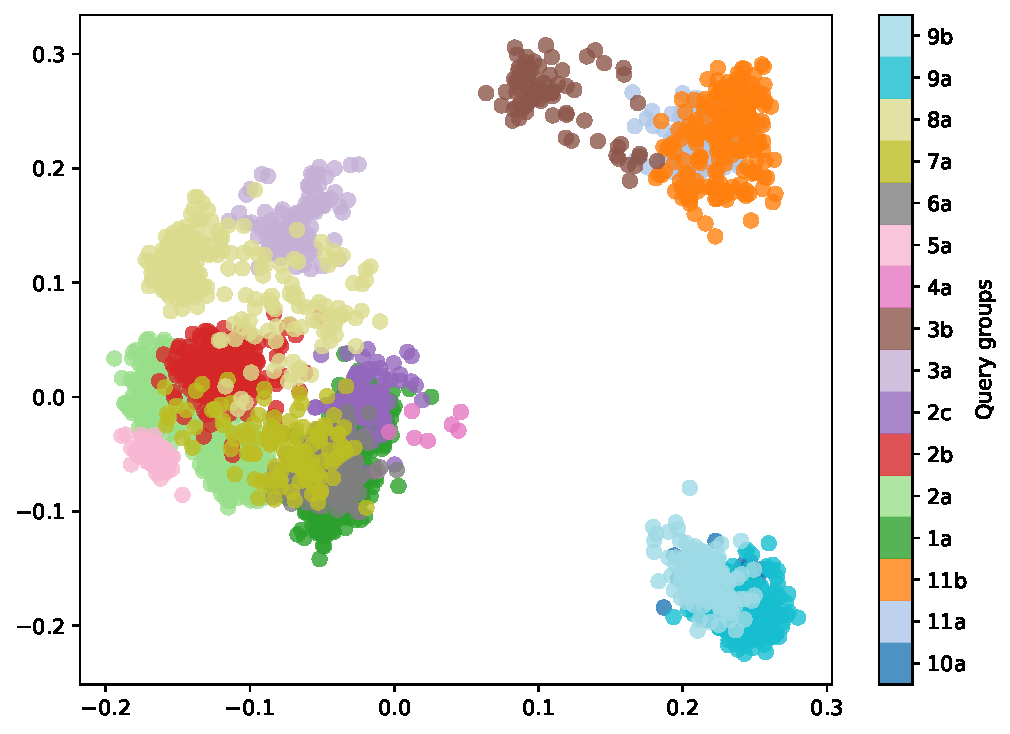
\includegraphics[width=0.5\linewidth]{images/pca_scatter.pdf} % расширение .pdf указывать не требуется
\caption{Стандартные планы после PCA}
\label{fig:pca_scatter}
\end{figure}

Эксперименты проводились на сервере с 128 CPU-ядрами на базе процессоров HiSilicon Kunpeng-920 и 1000ГБ оперативной памяти. Хранилище — SSD NVMe диском на 2ТБ, обеспечивающим высокие скорости чтения/записи для быстрого доступа к данным. Использовалась одноузловая база данных \emph{openGauss}. Были заданы следующие параметры конфигурации:

\begin{itemize}
    \item \texttt{shared\_buffers = 256 GB}
    \item \texttt{bulk\_write\_ring\_size = 10 GB}
    \item \texttt{work\_mem = 80 GB}
    \item \texttt{cstore\_buffers = 4 GB}
    \item \texttt{query\_dop = 1} (однопоточное выполнение запросов для лучшего контроля над производительностью)
\end{itemize}
Эксперименты выполнены на датасете IMDB, включающем 3133 запроса из рабочей нагрузки JOB--CEB. Набор основан на 16 шаблонах из оригинального бенчмарка JOB, причём каждый шаблон даёт различное число запросов. Эмбеддинги планов получены моделью OpenAI \texttt{text-embedding-3-large}; таким образом, для каждого запроса доступны стандартный и оптимизированный планы, их эмбеддинги и соответствующие времена выполнения.
На рис.~\ref{fig:pca_scatter} показано расположение стандартных планов после сведения размерности высокоразмерных эмбеддингов к двум главным компонентам методом главных компонент (PCA). Каждая точка соответствует одному плану, спроецированному на две главные компоненты, а цвет кодирует метку шаблона запросов (см. легенду).

Предыдущие исследования по PostgreSQL сообщают, что несколько отдельных подсказок способны ускорять нагрузку JOB--CEB более чем на 60~\%; например, глобальное отключение соединений вложенными циклами даёт такой прирост. В отличие от PostgreSQL, отключение того же оператора соединения в \emph{openGauss} ухудшает производительность примерно на 50~\%, существенно усложняя задачу выбора оптимального набора подсказок.
В табл.\ref{fig:hintset_combo}(a) перечислены десять самых частых \emph{оптимальных} наборов подсказок.
Примерно для половины запросов оптимальная конфигурация совпадает со стандартной (все операторы включены);
в сумме 86 из 128 возможных бит-векторов хотя бы раз оказывались оптимальными.
На рис.\ref{fig:hintset_combo}(b) показано глобальное распределение всех наблюдаемых наборов подсказок.
Лидеры разнообразны — отключение только \texttt{enable\_nestloop} \emph{не} всегда является лучшей стратегией.


\begin{figure}[htbp]
  \centering
  %======================= панель (a): таблица =======================
  \begin{minipage}[t]{0.48\linewidth}
    \centering
    \textbf{(a)}\\[4pt]               % отметка «(a)»
    \small                            % уменьшенный шрифт для таблицы
    \begin{tabular}{l r}
      \toprule
      Hintset & Count \\
      \midrule
      0000000 & 1468 \\
      0001100 & 226  \\
      1000100 & 146  \\
      1100100 & 114  \\
      0000100 & 106  \\
      0100100 & 46   \\
      0100000 & 45   \\
      0000001 & 43   \\
      1000000 & 41   \\
      0011100 & 40   \\
      \bottomrule
    \end{tabular}
  \end{minipage}%
  \hfill                              % чуть свободного пространства между панелями
  %======================= панель (b): гистограмма ===================
  \begin{minipage}[t]{0.48\linewidth}
    \centering
    \textbf{(b)}\\[4pt]
    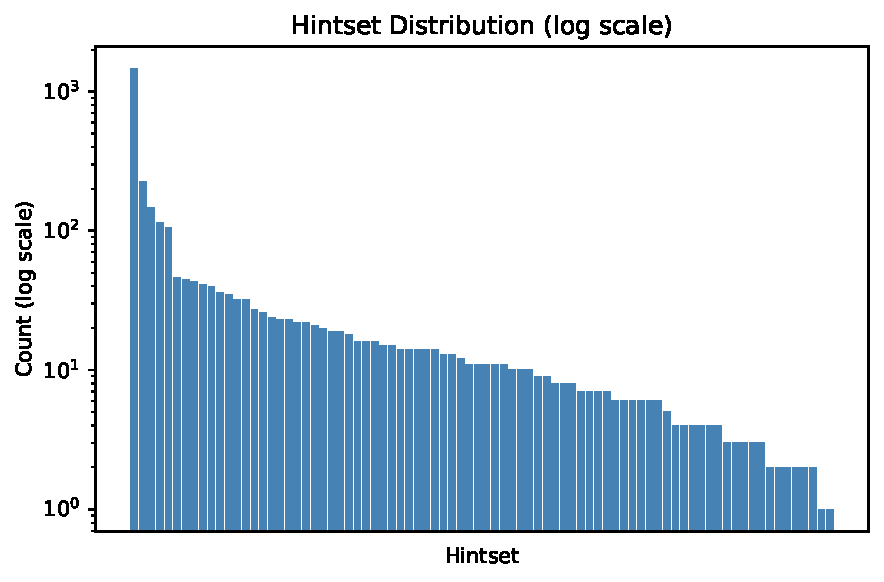
\includegraphics[width=\linewidth]{images/hintset_histogram_logscale}
  \end{minipage}

  \caption{Статистика для наборов хинтсетов: (a) Топ 10 наиболее часто встречающихся  хинтсетов и (b) распределение всех хинтсетов в логарифмическом масштабе.}
  \label{fig:hintset_combo}
\end{figure}

На рис.\ref{fig:combined}(a) суммированы итоги десятикратной кросс-валидации: в каждом фолде 10\% запросов JOB--CEB откладывались для тестирования, а оставшиеся 90~\% формировали эталонное хранилище для Plan-Mapping.

Совокупное время выполнения по десяти фолдам в среднем сократилось на \textbf{19{,}1~\%} (т.е. запросы в среднем выполняются в 1{,}19 раза быстрее стандартного оптимизатора). Прирост устойчив: даже самый слабый фолд дает +8\%, а лучший -- +32\%. Максимально достижимое ускорение для всей нагрузки — 62{,}5~\%. В \emph{среднем фолде} 20~\% запросов ускоряются, 20~\% замедляются, а оставшиеся 60~\% не меняются. Время 90-го перцентиля снижается на 24{,}7~\%, тогда как медиана улучшается умеренно — на 2{,}1~\%. 


\begin{figure}[htbp]
  \centering
  %========================= (a) рисунок ==========================
  \begin{minipage}[t]{0.51\linewidth}
    \centering
    \textbf{(a)}\\[4pt] % тут своя метка
    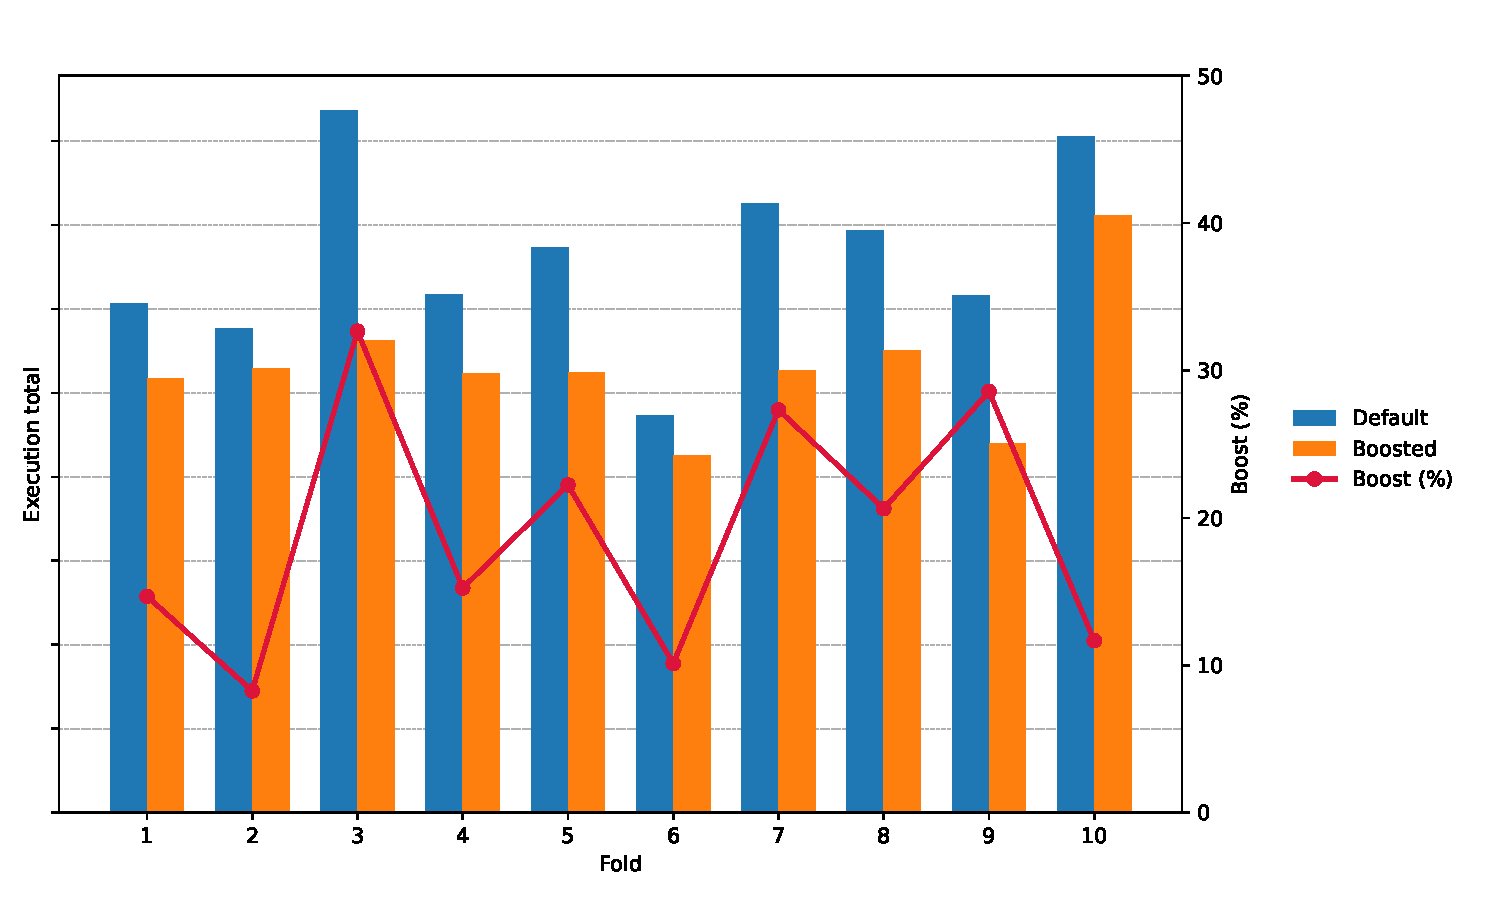
\includegraphics[width=0.9\linewidth]{images/infographic}
  \end{minipage}%
  \hfill
  %========================= (b) таблица ==========================
  \begin{minipage}[t]{0.48\linewidth}
    \centering
    \textbf{(b)}\\[4pt] % и тут
    \footnotesize
    \begingroup                             % локальное изменение табличных интервалов
      \setlength{\tabcolsep}{5pt}           % было 6 pt
      \renewcommand{\arraystretch}{1.0}     % высота строк (если нужно ≈0.9–1.0)

      %---- таблица -------------------------------------------------
      \begin{tabular}{l@{\hspace{5pt}}r@{\hspace{5pt}}r@{\hspace{5pt}}r}
        \toprule
        \shortstack[l]{Верхняя\\граница\\перцентил}
          & \shortstack[c]{Среднее\\стандартное\\время}
          & \shortstack[c]{Среднее\\ускоренное\\время}
          & Ускорение\% \\
        \midrule
        0.1 &   564   &   628   & -11 \\
        0.2 &  1658   &  1651   &   0 \\
        0.3 &  2812   &  2740   &   3 \\
        0.4 &  4203   &  4096   &   3 \\
        0.5 &  6144   &  5954   &   3 \\
        0.6 &  8617   &  8293   &   4 \\
        0.7 & 12802   & 11681   &   9 \\
        0.8 & 19809   & 17059   &  14 \\
        0.9 & 35201   & 27923   &  21 \\
        1.0 & 121154  & 90734   &  25 \\
        \bottomrule
      \end{tabular}
      %--------------------------------------------------------------
    \endgroup
  \end{minipage}

  \caption{(a) Улучшение времени исполнения по фолдам для Plan-Mapping.
           (b) Разбиение среднего времени по перцентильным срезам и ускорение (\%).}
  \label{fig:combined}
\end{figure}

Таблица на рис.~\ref{fig:combined}(b) разбивает среднее время выполнения запросов на перцентильные интервалы. Столбец «Верхняя граница перцентиля» задаёт верхнюю границу каждого интервала; нижняя граница равна предыдущему перцентилю. Например, строка 0.5 охватывает срез 0.4–0.5. Столбцы «Стандартное» и «Ускоренное» показывают среднее время внутри среза, а «Ускорение» — процентное изменение в нём. Plan-Mapping даёт наибольший эффект в «длинном хвосте» — в срезах с самыми медленными запросами, хотя в некоторых быстрых срезах встречаются локальные замедления.

\subsection{Исследование абляций}
Естественный вопрос — дают ли обученные LLM-эмбеддинги реальную пользу сверх «дорогого сопоставления строк»? Чтобы ответить на него, мы повторили оценку в двух аблированных конфигурациях, где этап проверки согласованности был отключён. Это устраняет влияние дополнительной верификации и позволяет оценить, действительно ли эмбеддинги планов полезны для оценки близости планов по сравнению с простыми строковыми метриками:

\begin{enumerate}
\item \textbf{Расстояние Левенштейна} — кандидаты извлекаются исключительно по редакционному расстоянию Левенштейна;
\item \textbf{LLM-эмбеддинги (без проверки согласованности)} — то же, что и полная система, но без этапа проверки согласованности.
\end{enumerate}

В варианте с расстоянием Левенштейна мы не строим эмбеддинги и не сравниваем векторы по евклидовой метрике; вместо этого вычисляем редакционное расстояние
\[
d_{\text{lev}}(p_{1},p_{2})=\min_{\pi}\lvert\pi\rvert ,
\]
где $\pi$ - последовательность одиночных вставок, удалений или замен символов, преобразующих строку плана $p_{1}$ в строку плана $p_{2}$.  

Табл.\ref{tab:ablation-latency} показывает общий выигрыш по времени и число запросов, превысивших тайм-аут 450с.
Без проверки согласованности вариант с расстоянием Левенштейна не только не ускоряет нагрузку: он замедляет её на \textbf{64{,}4~\%} и приводит к \textbf{87} тайм-аутам.
Напротив, LLM-эмбеддинги всё ещё дают \textbf{16{,}1~\%} ускорения при всего \textbf{5} тайм-аутах — в пять раз меньше, чем у Левенштейна, и близко к стандартному оптимизатору (3).
При повторном включении проверки согласованности (разд.\ref{sec:ch3/sec2}) ускорение возрастает до \textbf{21{,}1\%}, а число тайм-аутов сокращается до одного запроса.

Эти наблюдения подтверждают, что обученные эмбеддинги захватывают информацию, значительно выходящую за рамки сырой строковой близости, и в сочетании с проверкой согласованности являются ключом к устойчивому приросту производительности.

\begin{table}[htbp]
  \centering

  
  \begin{tabular}{lccc}
    \toprule
                     & Только выбор подсказок
                     & Количество тайм-аутов \\
    \midrule
    Расстояние \\ Левенштейна      & $-64.4\%\;$
                     & 87  \\[2pt]
    LLM Эмбеддинги   & $16.1\%\;$
                     & 5  \\
    \bottomrule
  \end{tabular}

  \caption{Совокупное изменение времени исполнения (положительное = ускорение) и число тайм-аутов для каждой метрики расстояния}
    \label{tab:ablation-latency}
\end{table}

В главе представлен подход переноса оптимизационных подсказок по эмбеддингам планов. Система строит векторные представления планов, находит ближайших соседей в репозитории опыта, извлекает устойчивые наборы подсказок и применяет их через строгую проверку согласованности и безопасности. Метод не требует длительного обучения — достаточно накопления опыта — и не зависит от конкретных групп запросов или изменений данных: при дрейфе нагрузки меняется ландшафт эмбеддингов и соседства, а валидация удерживает качество. Подсистема совместима с текущим планировщиком и не меняет его архитектуру.

Эксперименты показали устойчивое снижение времени выполнения прежде всего у хвостовых запросов — именно там выигрыш максимален. Цена применения умеренная. Перебор кандидатов остаётся дорогой операцией, а запрос планируется дважды — исходный план и план-кандидат. На стандартном JOB время планирования порядка 10\% от времени исполнения, поэтому двойное планирование почти не влияет на итоговое время. В JOB-CEB встречаются хвостовые запросы с большим временем выполнения — для них двойное планирование это малая плата за значимую оптимизацию. Подход нацелен на исправление хвоста и в меньшей степени на снижение медианного времени.

Исследование отдельных компонент метода подтвердили, что обученные LLM-эмбеддинги действительно полезны для предсказания подсказок. Однако даже современные эмбеддинги OpenAI обучены на крайне ограниченном материале, где планы запросов сочетаются с явной информацией о том, как подсказки на них влияют. Следующий шаг — предметные эмбеддинги, обученные на корпусах с богатым SQL, аннотациями подсказок и обратной связью по стоимости. Это усилит поиск соседей и расширит способность модели рассуждать о сложных паттернах оптимизации.

Текущий конвейер даёт среднее ускорение около 20\% — примерно треть теоретического максимума на данной нагрузке — и при этом выявляет очевидные точки роста. Около половины оставшегося разрыва приходится на этап выбора кандидатных подсказок. В конфигурации с точным предсказанием, где проверка согласованности видит истинные времена и базового, и кандидатного планов, удаётся вернуть почти 40\% потенциального ускорения — две трети максимума. Это указывает, что более изощрённая метрика сходства или голосование на первом этапе способны закрыть значимую часть остаточного зазора.

Гетерогенность движков и железа не позволяет полагаться на «универсальные» подсказки. Для PostgreSQL сообщалось о среднем ускорении свыше 60\% от одной подсказки «запретить соединение вложенными циклами», тогда как на openGauss та же подсказка приводит к ухудшению более чем на 50\%. Это мотивирует стратегию нескольких окрестностей и отказ от единой догмы — подсказка должна подтверждаться локальным контекстом и проверками безопасности.

В следующей главе будет представлен улучшенный метод адаптивного поиска подсказок на основе LLM-агента. Он сокращает число запусков запросов по сравнению с адаптивным поиском из главы 3, быстрее находит устойчивые улучшения и экономит бюджет экспериментов.
\FloatBarrier
